\section{Measuring platform}

The method of using a shunt resistor was chosen to measure the energy consumption of the GPS. The shunt resistor was chosen due to its simple and cheap design but yet its low error rate compared to the Hall effect IC. The other software estimation techniques and cycle aware techniques were not chosen as they either tries to estimate the energy consumption with poor accuracy or they need non available RTL level information about the design. The shunt resistor threats the system that is getting measured as a black box, which enables the measuring platform to be used with any system.  Figure \ref{fig:deploy} shows the deployment diagram of the measuring platform that is used. 

\begin{figure}[H]
\centering
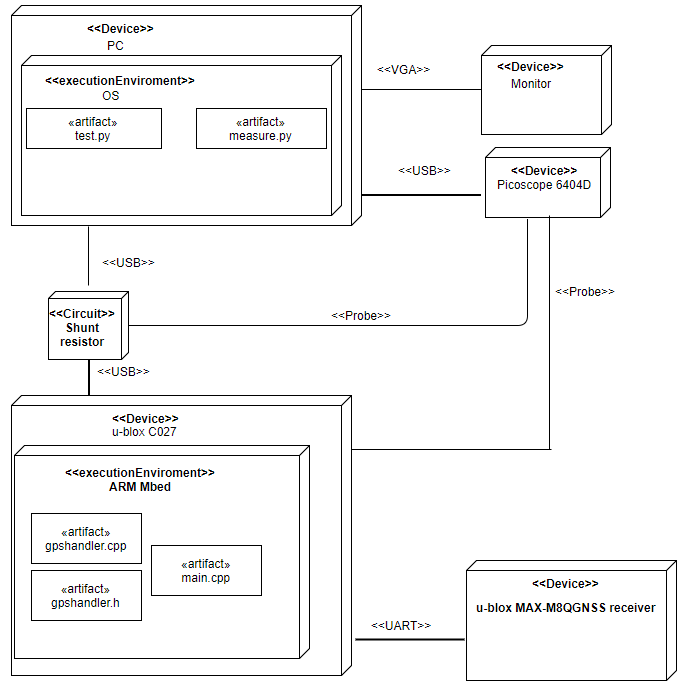
\includegraphics[height=4.5cm]{Project_Report/Images/deploy.PNG}
\caption{The deployment diagram for the rig that is used for measuring the energy consumption}
\label{fig:deploy}
\end{figure}

The platform consist of a micro controller with an embedded GPS, a digital oscilloscope, a shunt resistor, and a PC. The platform is mounted inside a box on a cycle wagon to make the platform mobile. The following section will highlight each parts task. 

\subsection{LoPy with Pytrack}
The LoPy is a micro controller equip with a LoRa, Wifi and BLE technology \cite{LoPy} and is specifically made for IoT use cases. It uses the Espressif ESP32 chip and the user write the program code in Micropython. LoPy has a low-power feature which makes it only use 25uA while still having some its internal peripheral on. The micro controller has UART,SPI, I2C and up to 24 GPIO.\\ The LoPy is equipped with Pycom's Pytrack, which is an extension shield to the LoPy. Pytrack is equipped with a L76-l GPS reciever from Quectel and a 3 axis 12 bit accelerometer \cite{Pytrack}. L76-l is a low power GNSS receiver with have many advanced power saving modes \cite{L76}. The module is equipped with an ARM7 processor and UART for serial communication. The LoPy controls the receiver through the execution of the program code and communicates with the Pytrack through serial communication. TTFF for the receiver is:
\begin{itemize}
\item Cold start:35s
\item Warm start: 30s
\item Hot start: 1s

\end{itemize}



\subsection{Shunt resistor}
\subsection{PC}
A Python script that uses the SDK from Picoscope is executed on the PC. The script is a modified version of Amen Hussain's energy measure script \cite{Amen}.  The scripts measures the energy consumption and plots the data to an Outlook file. The script is included in the appendix. 


\subsection{PicoScope 640 AD}
PicoScope 6000 from Picotecnology is a 4 channel digital oscilloscope with 5GS/s sampling and 2 GSample buffer memory \cite{Pico}. The oscilloscope is equipped with USB 3.0 and supplied with an SDK that enables the user to write their own software. The PicoScope has advanced trigger possibilities and a bandwidth of 500MHz along with a signal generator. The oscilloscope is used to measure the voltage drop across the shunt resistor.  

\newpage